\documentclass[masters,online,forcegraphics,final]{ruthesis}
%%%%%%%%%%%%%%%%%%%% TeXStudio Magic Comments %%%%%%%%%%%%%%%%%%%%%
%% These comments that start with "!TeX" modify the way TeXStudio works
%% For details see http://texstudio.sourceforge.net/manual/current/usermanual_en.html   Section 4.10
%%
%% What encoding is the file in?
% !TeX encoding = UTF-8
%% What language should it be spellchecked?
% !TeX spellcheck = en_US
%% What program should I compile this document with?
% !TeX program = xelatex

%%%%%%%%%%%%%%%%%%%% Bibliography options %%%%%%%%%%%%%%%%%%%%%
%% We suggest switching from bibtex to biblatex/biber because it is better able
%% to deal with Icelandic characters and other bibliography issues
%% As long as you use biblatex instead of bibtex by itself, it will at least
%%  generate a document without errors.
%% !!!If you are using TeXStudio, don't forget to update the bibliography setting!!!
\usepackage[backend=biber,bibencoding=utf8,style=ieee]{biblatex}
%\DeclareLanguageMapping{american}{american-apa}  
% need to declare mapping for style=apa to alphabetize properly
% If you set backend=bibtex, it will use bibtex for processing (old way)
%    this can work with Icelandic characters, but you may get weird results.
%    bibtex does not know how to sort Þ and ð
% if you set backend=biber, you can use UTF8 characters such as Þ and
%     ð  but you will have to remember to switch from using bibtex to 
%     biber in your client
% If you use JabRef, make sure the file is encoded in UTF-8 which is
% not the default.

%% This tells TeXStudio to use biber
% !TeX TXS-program:bibliography = txs:///biber
%% This also sets the bibliography program for TeXShop and TeXWorks
% !BIB program = biber

\addbibresource{references.bib}
% Where is your reference library?

\IfFileExists{custom.sty}{\usepackage{custom}}{}

\setTitle{My Title}{MY TITLE}
\setDocumentType{Final Report}
\author{Firstname1~Lastname1, Firstname1~Lastname2}
\setCourse{T-411-MECH}
\setSchool{\MLSSE{}}
\whensigned{17}{\MLdec}{2015}

\finalifforcegraphics{hyperref} %hyperlinks even in draft mode
\usepackage[hidelinks]{hyperref} 
\begin{document}

\frontmatter{}
\frontcover{}
\enableindents{}
\starttables{}% setup formatting
\tableofcontents{}
\thesislistoffigures{}
\thesislistoftables{}
\starttext{}
%\listoffixmes{}
\chapter{Some Chapter}
\section{Some section}
\subsection{Some Subsection}
Some text goes here with a citation~\cite{adams84fish}.
\printbibliography{}
\appendix{}



\chapter{Runway Usage}\label{cha:RWY_usage}


\begin{figure}[h]
    \centering
    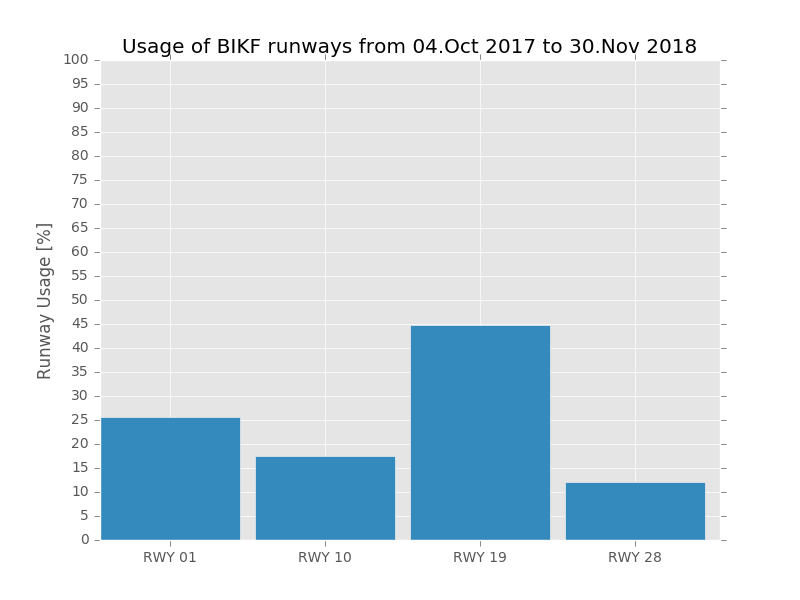
\includegraphics[width=0.8\textwidth]{graphics/fig_runway_usage_2017-10-04_to_2018-11-30.png}
    \caption[Runway usage at BIKF]{Overall runway usage at BIKF for a period of one year since October 2017. Almost half of all arrivals during that period (44,7\%) use RWY-19, followed by RWY-01 (25,7\%) and RWY-10 (17.6\%). The summer traffic favours RWY-19 with 52.8\%~(Figure~\ref{fig:runway_usage_summer}), while during the winter season some of those arrivals are diverted towards RWY-01 and RWY-10~(Figure~\ref{fig:runway_usage_summer}). RWY-28 is least used despite its fast-exit TWY B-1.}
    \label{fig:runway_usage}
\end{figure}


\begin{figure}[h]
    \centering
    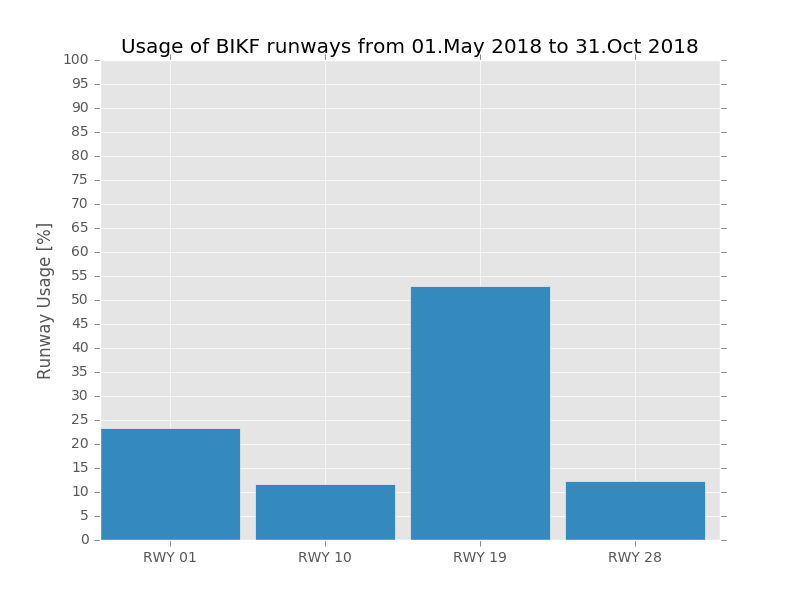
\includegraphics[width=0.7\textwidth]{graphics/fig_runway_usage_summer}
    \caption[Summer runway usage at BIKF]{The summer traffic favours RWY-19 (52,8\%), followed by RWY-01 (23,3\%), while RWY-10 and RWY-28 are with 11,6\% and 12,3\% respectively.}
    \label{fig:runway_usage_summer}
\end{figure}


\begin{figure}[h]
    \centering
    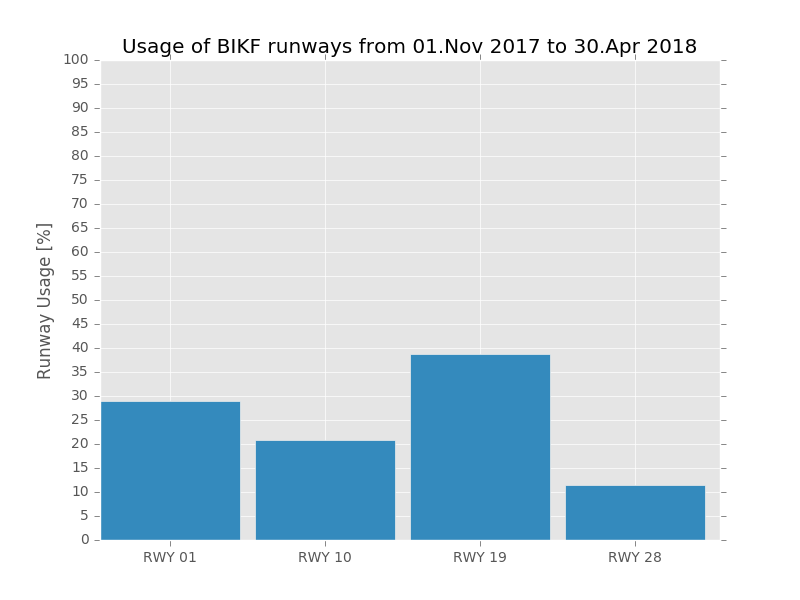
\includegraphics[width=0.7\textwidth]{graphics/fig_runway_usage_winter}
    \caption[Winter runway usage at BIKF]{The winter traffic at BIKF is a bit more evenly distributed among runways bit still favours RWY-19 (38,8\%),followed by RWY-01 with 28,9\%, RWY-10 (20,8\%) and RWY-28 (11,4\%).}
    \label{fig:runway_usage_winter}
\end{figure}


\chapter{Arrival Runway Occupancy Times\label{cha:AROTs}}


% Please add the following required packages to your document preamble:
% \usepackage{graphicx}
\begin{table}[h]
\centering
\resizebox{0.8\textwidth}{!}{%
\begin{tabular}{lr|r|r|r|r|r|r|r|}
\cline{3-9}
                          & \multicolumn{1}{c|}{}   & \multicolumn{7}{c|}{AROT [s]} \\ \hline
\multicolumn{1}{|l|}{RECAT-EU} & count & mean & std & min & 25\% & 50\% & 75\% & max \\ \hline
\multicolumn{1}{|l|}{CAT-A}    & 2     & 119  & 19  & 105 & 112  & 119  & 125  & 132 \\ \hline
\multicolumn{1}{|l|}{CAT-B}    & 53    & 81   & 20  & 51  & 65   & 77   & 91   & 136 \\ \hline
\multicolumn{1}{|l|}{CAT-C}    & 3436  & 78   & 17  & 46  & 65   & 75   & 89   & 155 \\ \hline
\multicolumn{1}{|l|}{CAT-D}    & 1029  & 75   & 18  & 46  & 62   & 71   & 87   & 155 \\ \hline
\multicolumn{1}{|l|}{CAT-E}    & 95   & 88   & 24  & 46  & 71   & 85   & 101  & 151 \\ \hline
\multicolumn{1}{|l|}{CAT-F}    & 49    & 84   & 22  & 48  & 72   & 81   & 91   & 155 \\ \hline
\end{tabular}%
}
\caption[AROTs for the air traffic mix by RECAT]{AROT statistics for the air traffic mix at BIKF by RECAT-EU categories. The count is the number of landings in peak hours since October 2017}
\label{tab:AROT_RECAT_stats}
\end{table}


% Please add the following required packages to your document preamble:
% \usepackage{graphicx}
\begin{table}[h]
\centering
\resizebox{\textwidth}{!} & \multicolumn{1}{l|}{50\%} & \multicolumn{1}{l|}{75\%} & \multicolumn{1}{l|}{max} \\ \hline
\multicolumn{1}{|l|}{Summer} & \multicolumn{1}{r|}{764} & 85 & 20 & 46 & 70 & 86 & 99 & 153 \\ \hline
\multicolumn{1}{|l|}{Winter} & \multicolumn{1}{r|}{263} & 100 & 17 & 55 & 87 & 98 & 111 & 156 \\ \hline
\end{tabular}%
}
\caption[AROTs RWY-01 pre fast exit by season]{AROTs for runway RWY-01 pre-fast-exit TWY A-1 by season}
\label{tab:season_AROT_stats_RWY01_pre_fast_exit}
\end{table}

% ----------------------------

% Please add the following required packages to your document preamble:
% \usepackage{graphicx}
\begin{table}[h]
\centering
\resizebox{\textwidth}{!} & \multicolumn{1}{l|}{50\%} & \multicolumn{1}{l|}{75\%} & \multicolumn{1}{l|}{max} \\ \hline
\multicolumn{1}{|l|}{Summer} & \multicolumn{1}{r|}{1879} & 84 & 22 & 46 & 64 & 86 & 98 & 152 \\ \hline
\multicolumn{1}{|l|}{Winter} & \multicolumn{1}{r|}{284} & 88 & 26 & 47 & 63 & 90 & 106 & 153 \\ \hline
\end{tabular}%
}
\caption[AROTs RWY-01 post fast exit by season]{AROTs for runway RWY-01 post-fast-exit TWY A-1 by season}
\label{tab:season_AROT_stats_RWY01_post_fast_exit}
\end{table}

% ----------------------------

% Please add the following required packages to your document preamble:
% \usepackage{graphicx}
\begin{table}[h]
\centering
\resizebox{\textwidth}{!} & \multicolumn{1}{l|}{50\%} & \multicolumn{1}{l|}{75\%} & \multicolumn{1}{l|}{max} \\ \hline
\multicolumn{1}{|l|}{Summer} & \multicolumn{1}{r|}{553} & 99 & 12 & 46 & 91 & 98 & 106 & 153 \\ \hline
\multicolumn{1}{|l|}{Winter} & \multicolumn{1}{r|}{249} & 110 & 13 & 60 & 100 & 108 & 117 & 155 \\ \hline
\end{tabular}%
}
\caption[AROTs RWY-28 pre fast exit by season]{AROTs for runway RWY-28 pre-fast-exit TWY B-1 by season}
\label{tab:season_AROT_stats_RWY28_pre_fast_exit}
\end{table}

% ----------------------------

% Please add the following required packages to your document preamble:
% \usepackage{graphicx}
\begin{table}[h]
\centering
\resizebox{\textwidth}{!} & \multicolumn{1}{l|}{50\%} & \multicolumn{1}{l|}{75\%} & \multicolumn{1}{l|}{max} \\ \hline
\multicolumn{1}{|l|}{Summer} & 401 & 68 & 14 & 49 & 60 & 66 & 72 & 155 \\ \hline
\multicolumn{1}{|l|}{Winter} & 69 & 73 & 13 & 49 & 63 & 72 & 79 & 105 \\ \hline
\end{tabular}%
}
\caption[AROTs RWY-28 post fast exit by season]{AROTs for runway RWY-28 post-fast-exit TWY B-1 by season}
\label{tab:season_AROT_stats_RWY28_post_fast_exit}
\end{table}



\begin{figure}
    \centering
    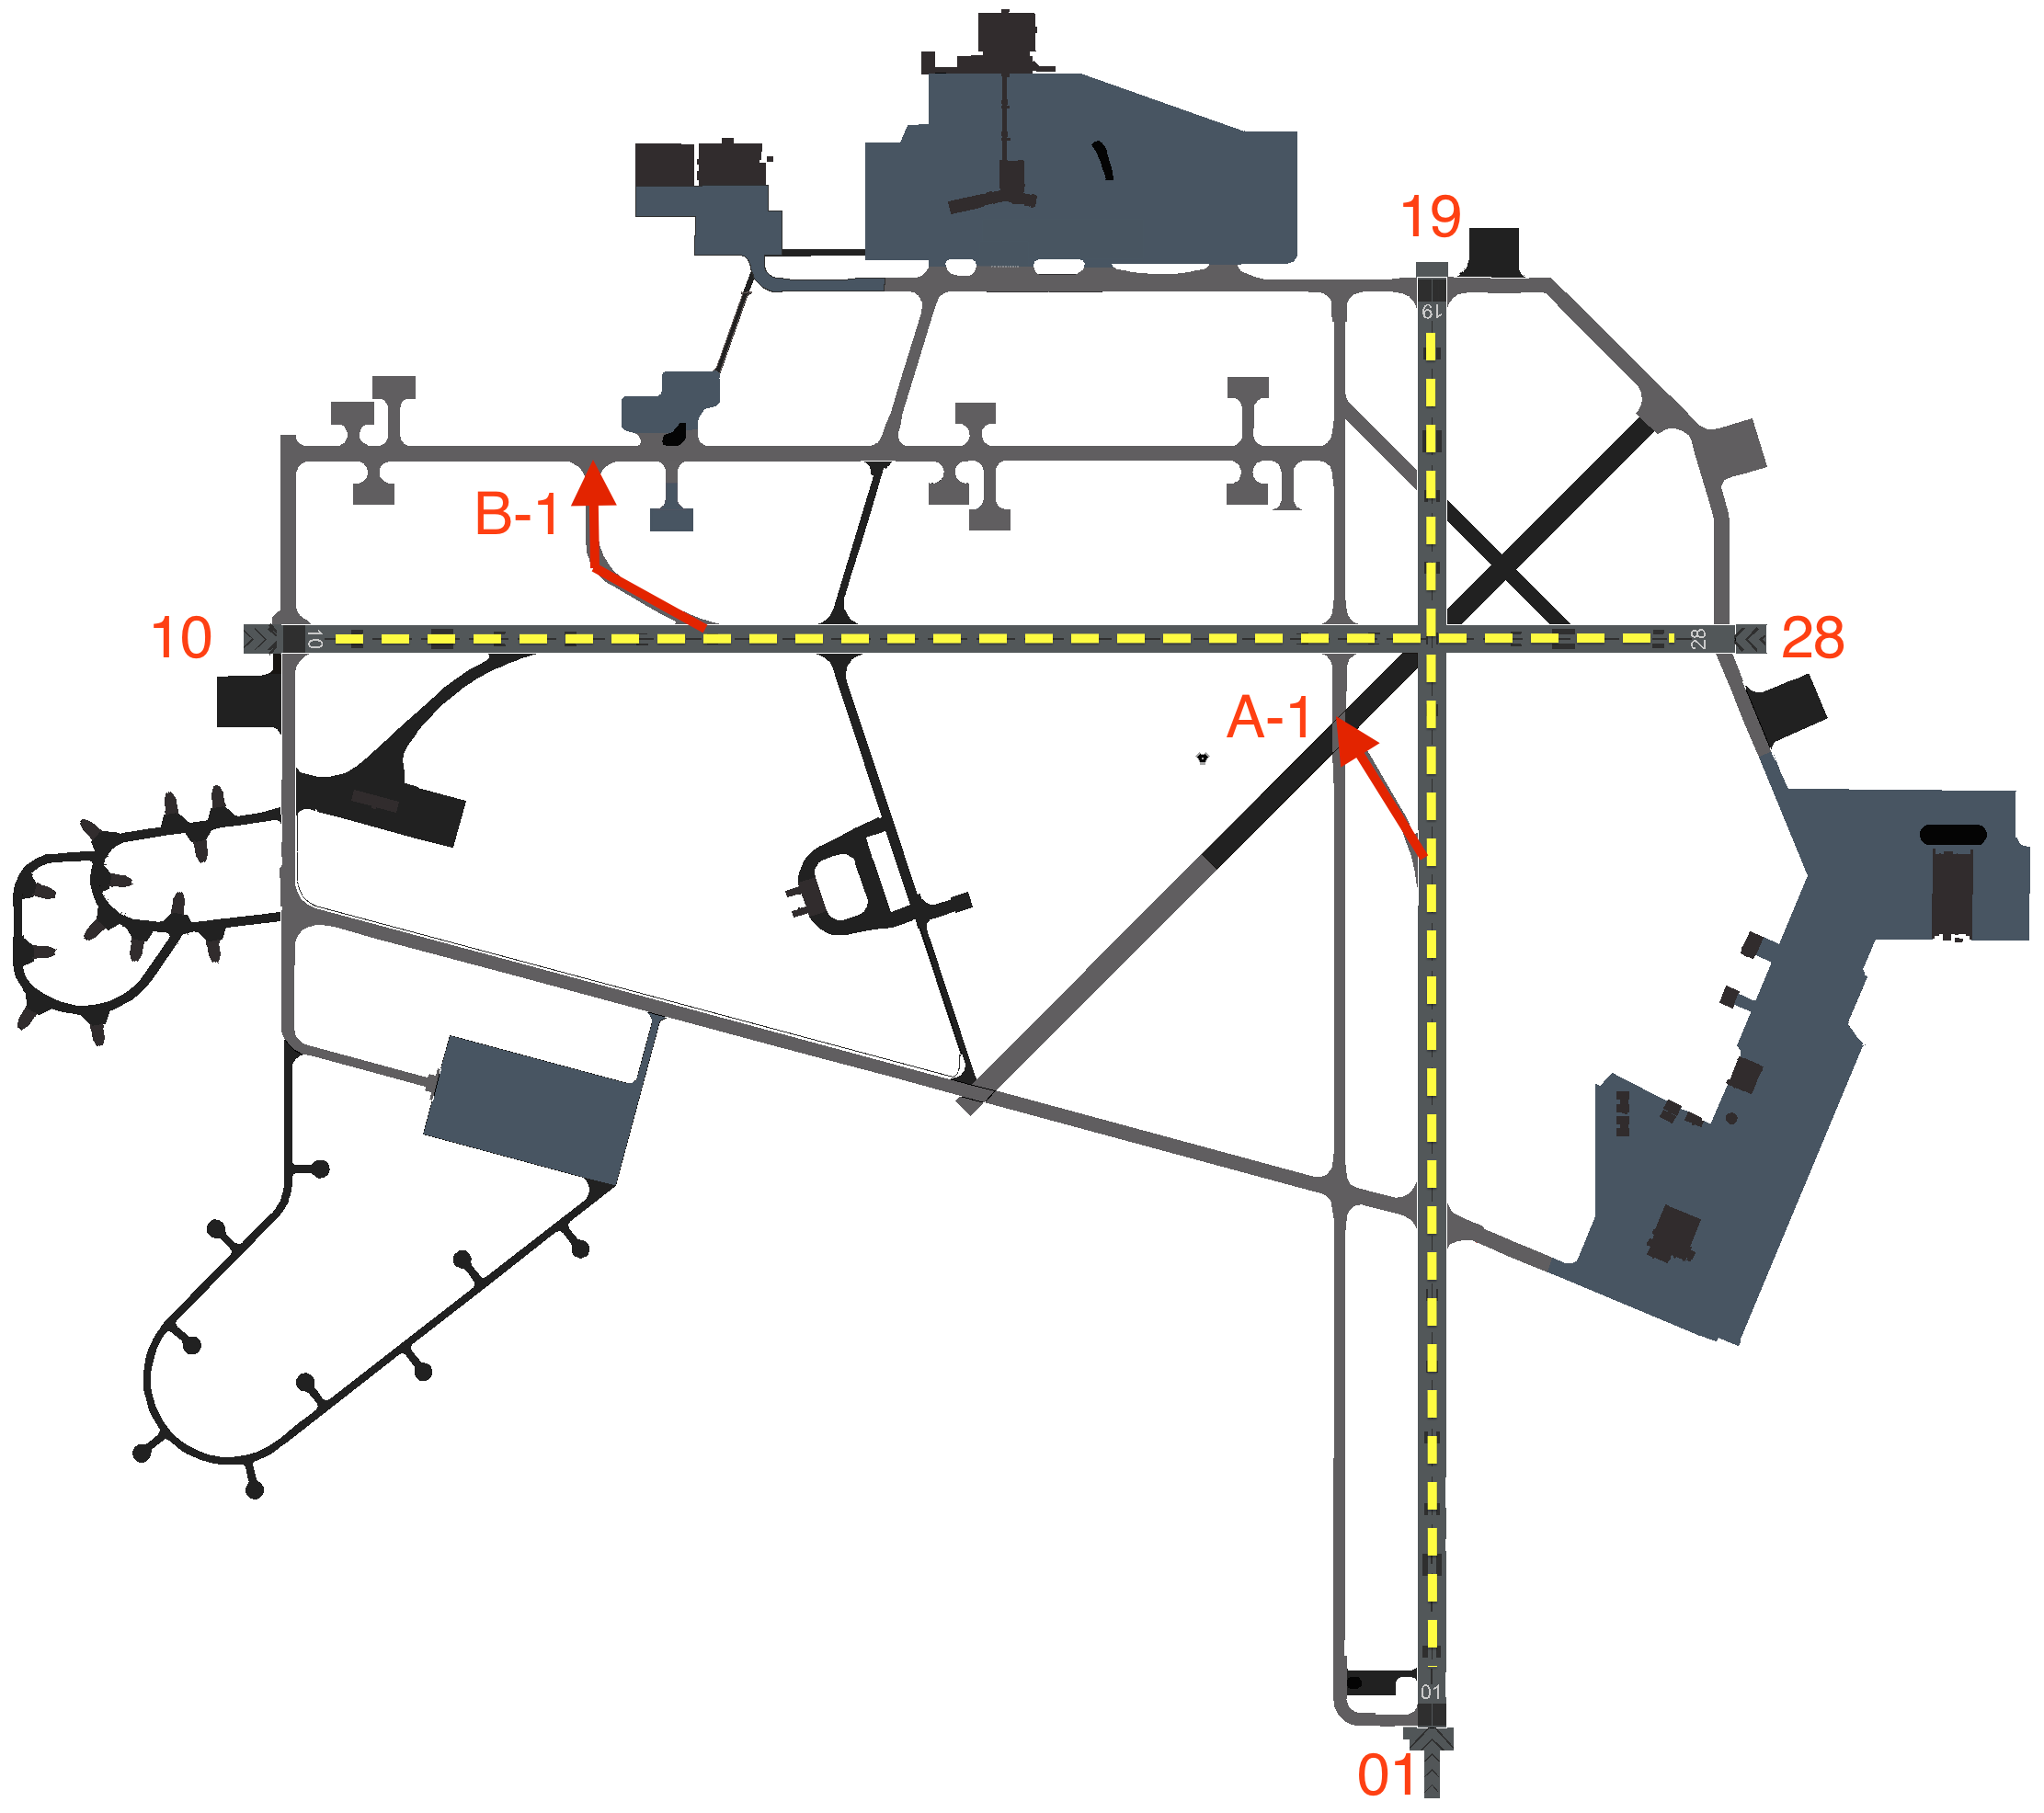
\includegraphics[width=1\textwidth]{graphics/BIKF_schematic.png}
    \caption[BIKF schematic]{BIKF schematic with marked runways and fast-exit taxiways.}
    \label{fig:BIKF_schematic}
\end{figure}
% ----------------------------


% \chapter{Code}\label{cha:code}
% You can put code in your document using the listings package, which is
% loaded by default in \path{custom.tex}.  Be aware that the listings
% package does not put code in your document if you are in draft mode
% unless you set the \texttt{forcegraphics} option.

% There is an example java (Listing~\ref{src:Data_Bus.java}) and XML
% file (Listing~\ref{src:AndroidManifest.xml}).  Thanks to the
% \texttt{url} package, you can typeset OSX and unix paths like this:
% \path{/afs/rnd.ru.is/project/thesis-template}.  Windows paths:
% \path{C:\windows\temp\ }.  You can also typeset them using the menukey
% package, but it tends to delete the last separator and has other
% complications.\footnote{The menukey package has issues with biblatex,
%   read \path{custom.tex} for more information.}

% If you are trying to include multiple different languages, you should
% go read the documentation and set these up in \path{custom.tex}.  You
% will save yourself a lot of effort, especially if you have to fix
% anything.

% %I have put the source code in the \directory{src/} folder.
% \lstinputlisting[language=Java, firstline=1,
% lastline=40, caption={Data\_Bus.java: Setting up the class.},
% label={src:Data_Bus.java}]{src/Data_Bus.java}

% \lstinputlisting[language={[android]XML}, firstline=1, lastline=20,
% caption={AndroidManifest.xml: Configuration for the Android UI.},
% label={src:AndroidManifest.xml}]{src/AndroidManifest.xml}

%%% Local Variables: 
%%% mode: latex
%%% TeX-master: "DEGREE-NAME-YEAR"
%%% End: 
 % as an example, perhaps some of your code
\clearforchapter{}
\printindex{}
\backcover{}
\end{document}


%%% Local Variables:
%%% mode: latex
%%% TeX-master: t
%%% TeX-engine: xetex
%%% End:
